%%%%%%%%%%%%%%%%%%%%%%%%%%%%%%%%%%%%%%%%%%%%%%%%%%%%%%%%%%%%%%%%%%%%%%%%%%
%%%%%%%%%%%%%%%%%%%%%%%%%%%%%%%%%%%%%%%%%%%%%%%%%%%%%%%%%%%%%%%%%%%%%%%%%%
\section{Appendix: Study of Relaxing the Dijet Invariant Mass Cut on aTGC limits}
\label{sec:afmufsucrosschecks}
% ---- ---- ---- ---- ---- ---- ---- ---- ---- ---- ---- ---- ---- ---- ----

A study was performed to assess the impact of increasing the dijet invariant mass
window size on the upper limits calculated for the anomalous triple gauge coupling
parameters.

The inputs described in Sec.~\ref{sec:atgc} were recalculated by
relaxing the window to $70 < m_{jj} < 100$~\GeV, and the limit
computation was performed for the non-b-tag channels on these modified
inputs. The results are shown in Fig.~\ref{fig:atgc2dlim_largemjjwin}.

\begin{figure}[bthp]
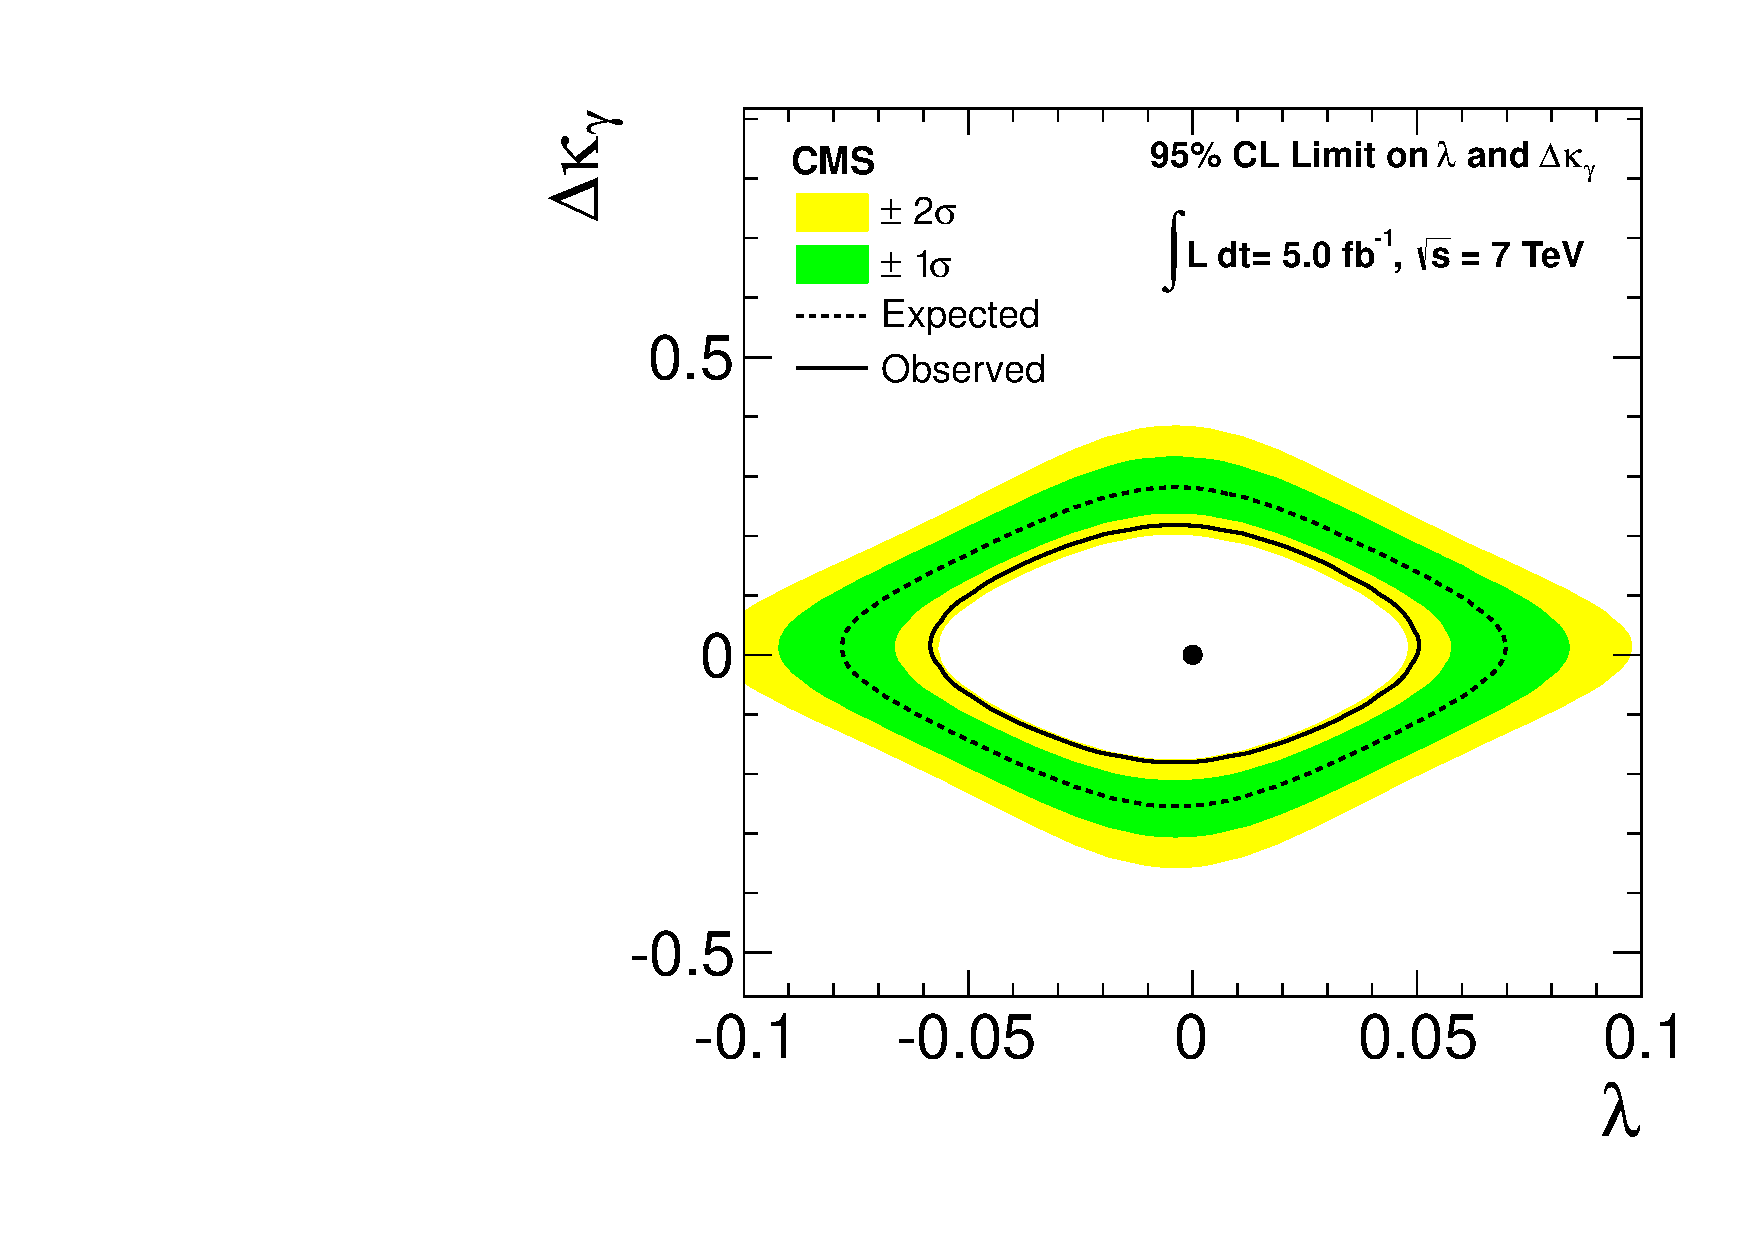
\includegraphics[width=0.8\textwidth]{figs/lz_dkg_2dlimit_largemjjwin.pdf}
\caption{\label{fig:atgc2dlim_largemjjwin} The observed and expected
values of the shape-based CL${}_{\textrm{S}}$ limit for anomalous
triple gauge couplings in $\lambda_Z:\Delta{\kappa_\gamma}$ plane for
the non-b-tag channels. The dijet invariant mass window size was
increased relative to Fig.~\ref{fig:limitshape2d2ch}.  }
\end{figure}

The non-exclusion region has grown substantially with respect to
Fig.~\ref{fig:limitshape2d2ch}, because the relaxation of the invariant
dijet mass requirement allows in much more background than signal, 
degrading the upper limit.

\clearpage
